\documentclass[a4paper, 11pt]{article}%
\usepackage[T1]{fontenc}%
\usepackage[utf8]{inputenc}%
\usepackage{lmodern}%
\usepackage{textcomp}%
\usepackage{lastpage}%
\usepackage{graphicx}%
%
\newcommand\tab[1][1cm]{\hspace*{#1}}%
\usepackage{fullpage}%
\usepackage{graphicx}%
%
\begin{document}%
\normalsize%
\noindent%
\large\textbf{Diamond Light Source Ltd} \hfill\large\textbf{Date: \today}%
\\\normalsize Beam Diagnostics Group \hfill\\%
\\\\
\includegraphics[width = 1\textwidth]{./Latex_Report/Logo.PNG}\\\\%
\section*{BPM Test Report}%
This is a \LaTeX test report for the, beam profile monitor electronics that are used at Diamond. In this document the different tests will be recorded in their own individual section. along with the specific parameters that are being tested and the test method used.\\\\%
\clearpage%
\tableofcontents%
\listoffigures%
\clearpage%
\section{beam\_position\_raster\_scan}%
This is a template test\\\\%
\textbf{The devices used for this test are:}\\\\%
RF Source Rigol Technologies,DSG3030,DSG3B174500308,00.01.06\\%
Libera BPM with the Epics ID "TS-DI-EBPM-04:" and the MAC Address "00:d0:50:31:03:b9"\\%
RC4DAT-6G-95\\%
\\%
\textbf{The parameters used in this test are:}\\\\%
Fixed RF Output Power: -20 dBm\\%
Fixed Rf Output Frequency: 499.6817682 MHz\\%
Maximum Attenuation: 10 dB\\%
Minimum Attenuation: 5 dB\\%
Steps between min and max attenuations: 5\\

%


\begin{figure}[htbp]%
\centering%
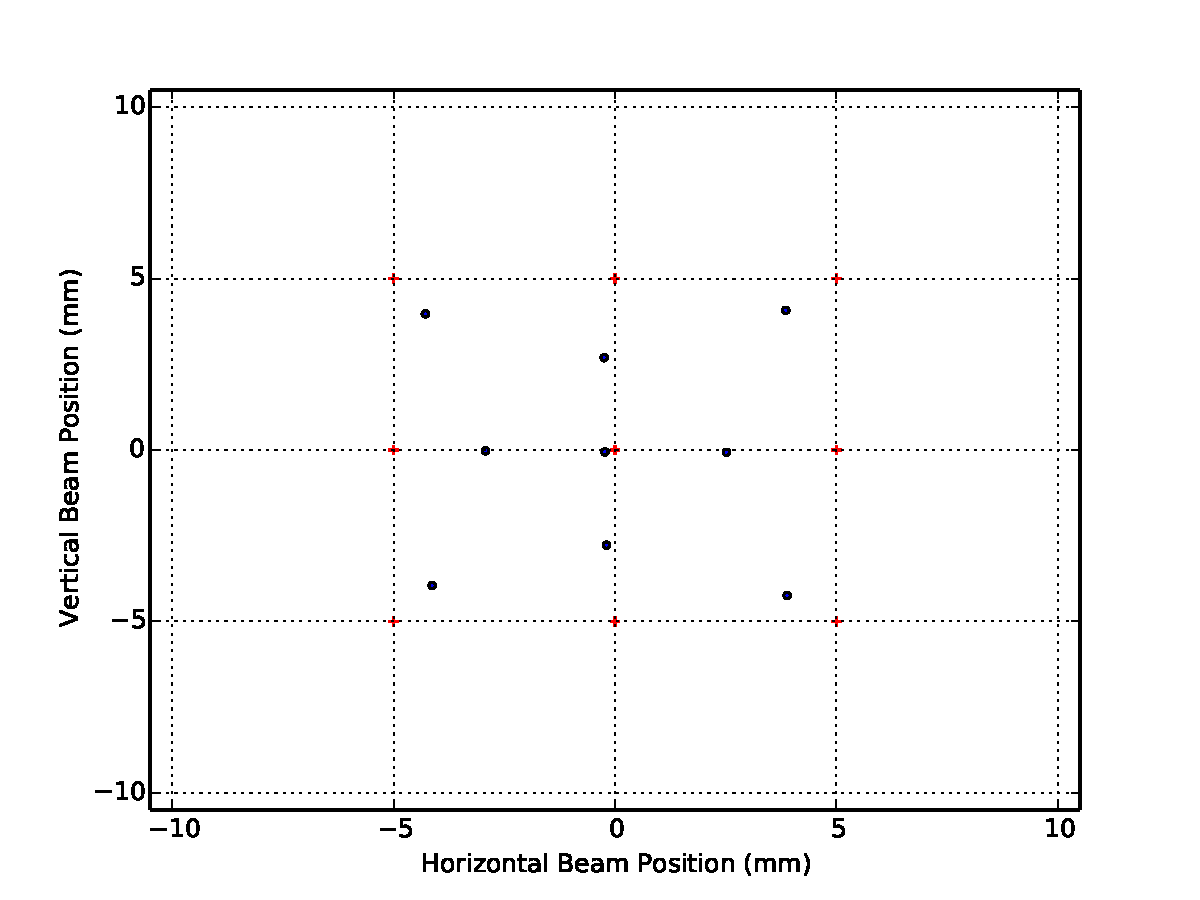
\includegraphics[width=0.8\textwidth]{beam_position_raster_scan}%
\caption{}%
\end{figure}

%
\end{document}